\documentclass[tikz]{standalone}
\begin{document}

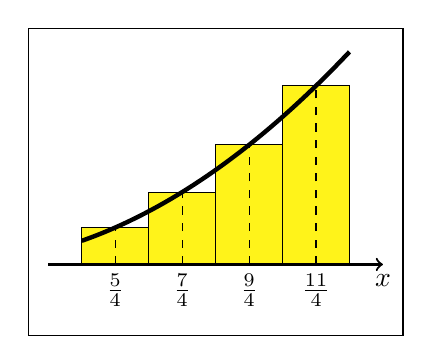
\begin{tikzpicture}[xscale=1.7,yscale=0.3]

  % create a white background, with a black frame
  \draw [fill=white] (0.6,-3) rectangle (3.4,10); 

  %% draw a grid
  %\draw[step=2mm, lightgray, thin] (-0.5,-0.7) grid (5.5,1.99); 
  %\draw[step=1cm, gray] (-0.5,-0.7) grid (5.5,1.99); 

  % draw Riemann Sum - Midpoint rule 
  \foreach \x in { 1,1.5,2,2.5} {
    \draw [fill=yellow!90] (\x,0) rectangle +(0.5,{(\x+0.25)*(\x+0.25)});
  }

  % draw axes
  \draw [->,thick] (0.75,0) -- (3.25,0) node[below] {$x$}; 

  % tick marks
  \foreach \x in {5, 7,9,11}{
    \draw [thick] (0.25*\x cm,-1pt) -- (0.25*\x cm,1pt) node[below]{$\frac{\x}{4}$};
    \draw [dashed] (0.25*\x cm,0) -- (0.25*\x cm,\x*\x/16);
    }

  % plot function
  \draw [ultra thick,smooth,variable=\x] plot [domain=1:3] (\x,\x*\x);

\end{tikzpicture}
\end{document} 
